\chapter{Resultados - Dados Experimentais}\label{cap_resul}

Neste capítulo serão apresentados os resultados obtidos através da
aplicação da metodologia proposta para sinais medidos no detector
ATLAS. Os sinais utilizados são divididos em dois tipos.
Inicialmente, será verificada a capacidade dos algoritmos
propostos para identificar (e consequentemente eliminar) os sinais
induzidos no detector por raios cósmicos. A seguir, serão
utilizados dados medidos no detector na fase inicial de operação
do LHC, onde a energia total dos feixes está limitada a 7 TeV
(funcionando em plena capacidade, o LHC atingirá energias da ordem
de 14 TeV).

Na Figura \ref{fig_evEJet} pode-se visualizar um evento (colisão)
do LHC onde foram gerados um elétron e três jatos. O elétron está
marcado em vermelho e aponta para baixo. Percebe-se que o elétron
não sensibiliza a seção hadrônica (pequenos quadrados em tons mais
escuros ou em amarelo indicam a sensibilização dos calorímetros)
\footnote{Neste diagrama, o calorímetro eletromagnético e o
hadrônico estão marcados respectivamente de verde e avermelhado.}.
Os jatos são representados pelos conjuntos de linhas adjacentes
que depositam energia na seção hadrônica do calorímetro. A linha
tracejada indica a direção onde foi detectada a ocorrência de
$E_{Tmiss}$ (falta de energia transversa).

Um outro evento do LHC visualizado pelo ATLAS é mostrado na
Figura~\ref{fig_evMu}, neste caso, pode-se observar dois múons,
que possivelmente foram gerados do decaimento de um bóson Z. É
interessante notar que somente os múons ultrapassam os
calorímetros, atingindo as câmaras de múons, que ficam na região
mais externa do detector.

\begin{figure}[th]
\centering
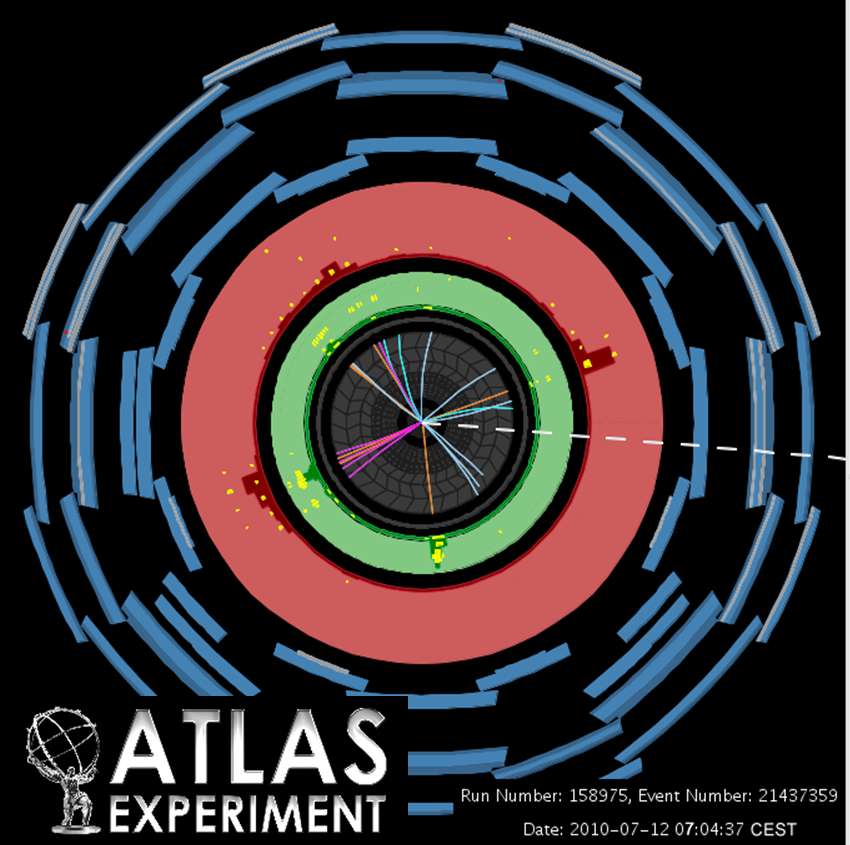
\includegraphics[width=11cm]{event_e_jet}
\caption[Visualização de um evento do LHC (7 GeV) onde foram
produzidos um elétron e três jatos.]{Visualização de um evento do
LHC (energia total dos feixes igual a 7 GeV) onde foram produzidos
um elétron (marcado em vermelho, apontando para baixo) e três
jatos, extraído de \cite{Homepage:ATLAS}.} \label{fig_evEJet}
\end{figure}

\begin{figure}[th]
\centering
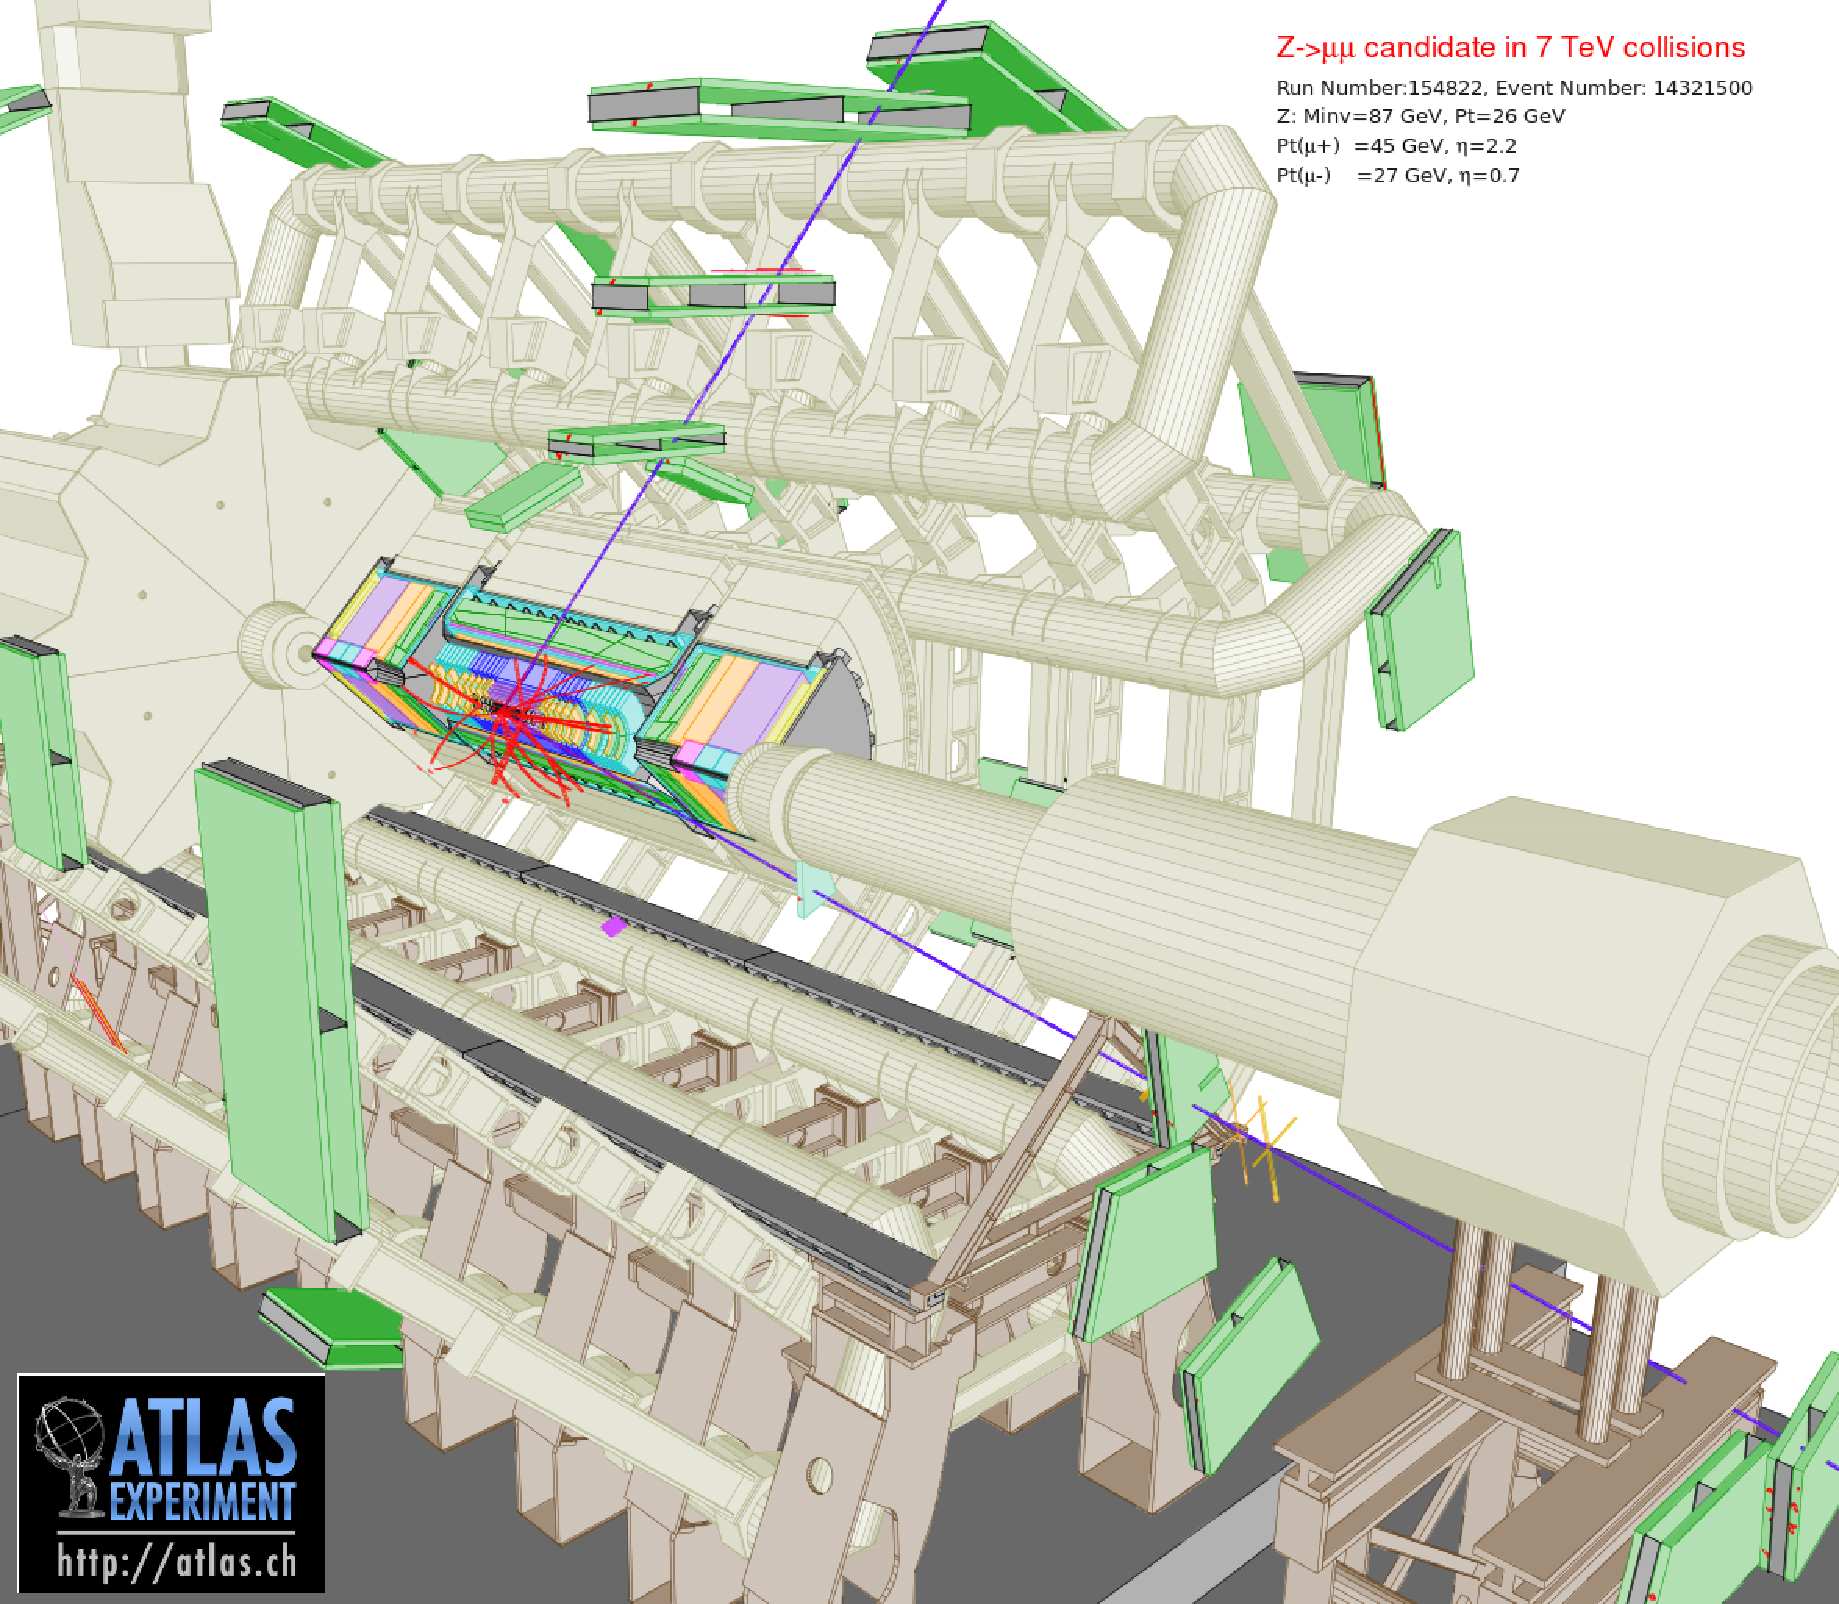
\includegraphics[width=15cm]{event_Z_mm}
\caption[Visualização de um evento do LHC (7 GeV) onde foram
produzidos dois múons a partir do decaimento de um bóson
Z.]{Visualização de um evento do LHC (energia total dos feixes
igual a 7 GeV) onde foram produzidos dois múons a partir do
decaimento de um bóson Z, extraído de \cite{Homepage:ATLAS}.}
\label{fig_evMu}
\end{figure}

\section{Validação com Sinais de Raios Cósmicos}

Os raios cósmicos \cite{book:cosmic:2002} são partículas
originadas no espaço, que se deslocam com velocidade próxima a da
luz. Ao penetrarem na atmosfera terrestre, interagem com os átomos
que a constituem produzindo uma "cascata" de novas partículas
menos energéticas (conhecidas como raios cósmicos secundários que
são compostos de diversas partículas, inclusive
múons~\cite{book:cosmicos:1990}). O poder de penetração dos raios
cósmicos é alto, podendo atingir o detector ATLAS (instalado a uma
profundidade de aproximadamente 100 m) e interagir com o material
dos calorímetros. Os raios cósmicos que chegam ao detector são
compostos essencialmente por múons. A energia destas partículas
pode ser alta, atingindo até $10^{20}$~eV.

Alguns estudos conduzidos no ATLAS estão interessados na análise
dos raios cósmicos, porém, considerando o canal elétron/jato, os
raios cósmicos constituem uma fonte de ruído de fundo, que deve
ser eliminada (ou pelo menos atenuada) pelo sistema de filtragem.
Em momentos quando o LHC está desligado (não havendo portanto
outra fonte de sinal para os calorímetros), foram coletadas
diversas assinaturas originadas por raios cósmicos, que serão
utilizadas para verificar a robustez do sistema de filtragem a
essa fonte de ruído. O conjunto utilizado é composto
de 26.347 eventos.

Na Figura \ref{fig_carcosmic}, pode-se observar a distribuição
destes eventos para diferentes valores de energia, $\eta$ e
$\phi$. Percebe-se que os eventos, embora concentrados abaixo de
100~GeV, podem atingir energia bastante elevada (até a ordem de
400~GeV, ocorrendo eventos isolados em 500~GeV e $\sim$1~TeV).
Devido à proveniência (direção de chegada) da radiação cósmica que
atinge o detector, a distribuição em $\eta$ não é uniforme,
havendo uma maior probabilidade destas partículas incidirem
perpendicularmente ao detector (produzindo valores baixos de
$\eta$). Considerando a distribuição em $\phi$, percebe-se uma
maior uniformidade.

\begin{figure}[h!]
\begin{minipage}[b]{0.48\linewidth}
  \centering
 \centerline{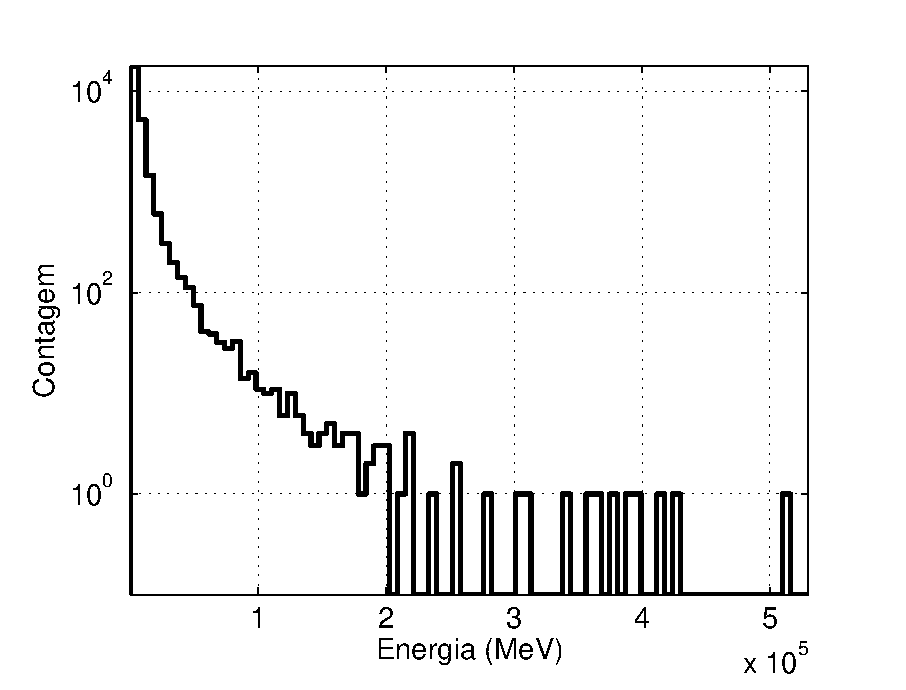
\epsfig{file=cosmics_et,width=8cm}}
\end{minipage}
\hfill
\begin{minipage}[b]{0.48\linewidth}
  \centering
 \centerline{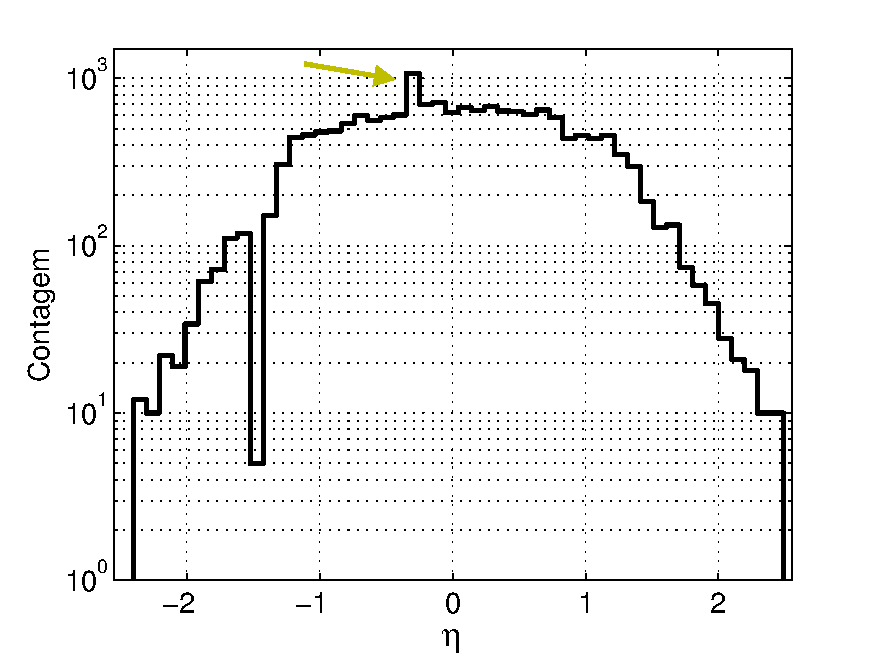
\epsfig{file=cosmics_eta,width=8cm}}
\end{minipage}
\hfill \linebreak
\begin{minipage}[b]{0.98\linewidth}
  \centering
 \centerline{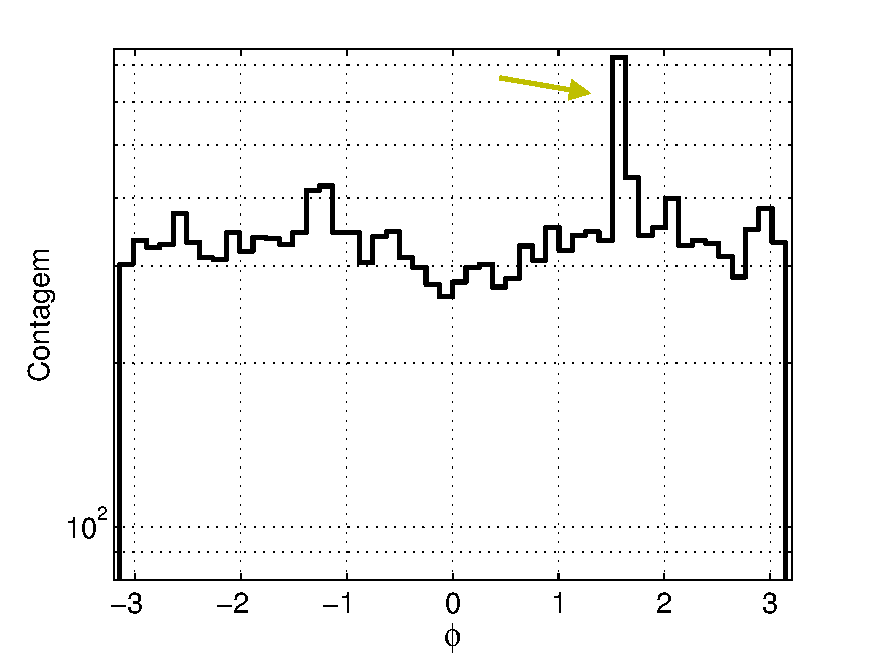
\epsfig{file=cosmics_phi,width=8cm}}
\end{minipage}
\caption{Histogramas em energia $\eta$ e $\phi$ dos eventos de
raios cósmicos.}\label{fig_carcosmic}
\end{figure}

Nos histogramas em $\eta$ e $\phi$, pode-se visualizar
um grande pico em cada um deles, correspondendo à região em torno
de ($\eta;\phi$)$=$(-0,3;1,6). Analisando-se o perfil de deposição
de energia nesta região, observou-se uma grande quantidade de
eventos que apresentam energia na camada E2, porém, nas outras
apenas ruído (um evento deste tipo é mostrado na
Figura~\ref{fig_cosmic_fant}). É muito improvável que um evento
físico real atravesse sete camadas do calorímetro e deposite
energia em apenas uma delas. Neste contexto, concluiu-se que,
estes eventos (chamados de eventos ``fantasmas'') foram gerados
por problemas nas células da segunda camada eletromagnética do
calorímetro, que, por algum motivo desconhecido, acusam a
deposição de energia mesmo quando nenhum evento foi recebido.

\begin{figure}[h!]
\begin{minipage}[b]{0.98\linewidth}
  \centering
 \centerline{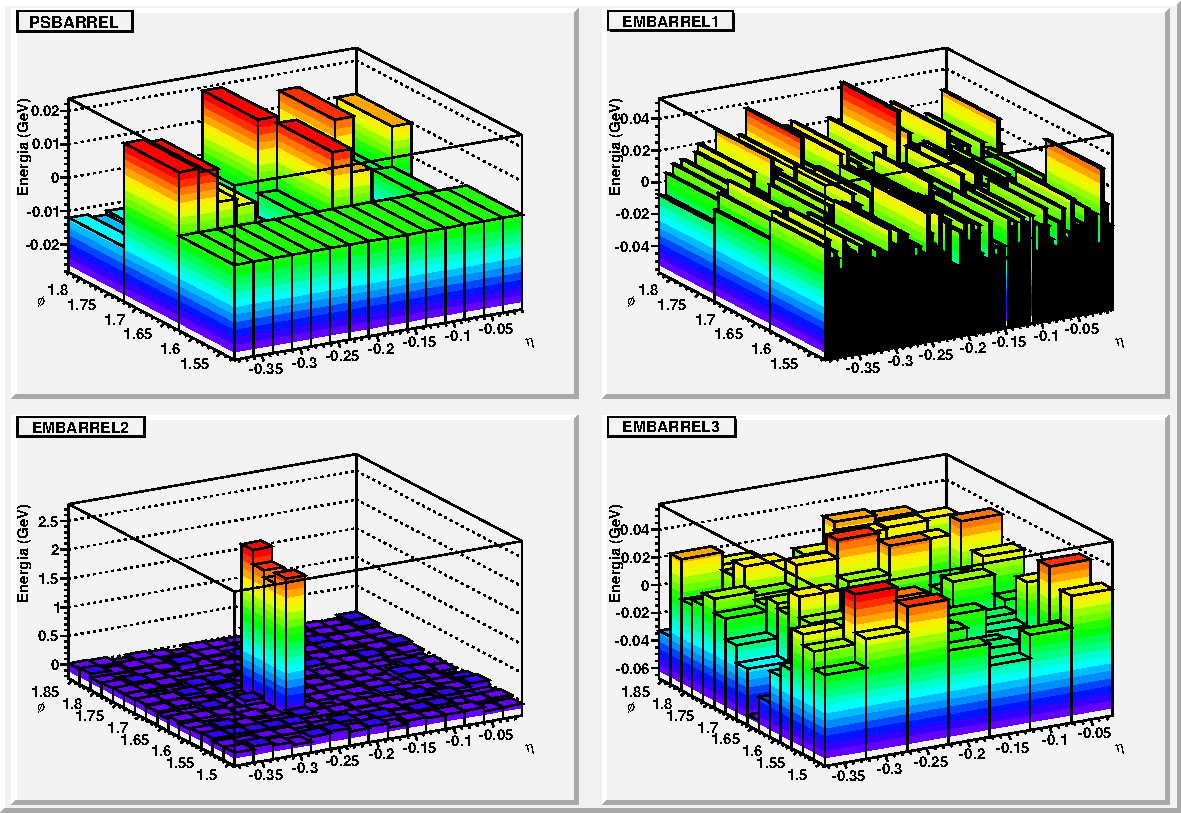
\epsfig{file=ev_cosmico_fant1,width=16cm}}
\end{minipage}
\caption[Exemplo de evento fantasma em
($\eta;\phi$)$=$(-0,3;1,6).]{Exemplo de evento fantasma em
($\eta;\phi$)$=$(-0,3;1,6), retirado
de~\cite{tese:torres:2010}.}\label{fig_cosmic_fant}
\end{figure}

Considerando a física envolvida no processo de interação dos raios cósmicos (que são compostos essencialmente por
múons), espera-se que a maior parte
dos eventos seja facilmente rejeitada pelos discriminadores. Porém, em alguns casos raros,
múons podem interagir com o calorímetro produzindo fótons e pares $e^-e^+$. Estes
eventos seriam capazes de produzir um perfil de deposição de energia semelhante ao de elétrons, confundindo o
sistema de filtragem.

\subsection{Eficiência dos Sistemas de Classificação Propostos na Rejeição de Raios Cósmicos}

Para avaliar a eficiência de classificação dos raios cósmicos foi realizado um estudo comparativo entre
diferentes discriminadores. Para o T2Calo e o \emph{Neural Ringer} foram utilizadas versões destes algoritmos
implementadas no sistema de \emph{software} do detector (Athena). Considerando os discriminadores
baseados em componentes independentes (ICA e NLICA), foram empregadas versões treinadas para o conjunto
de elétrons e jatos com corte E10 (pois esse conjunto, comparado ao E15i, apresenta maior estatística em
eventos de energias mais baixas).

A Tabela~\ref{tab_cosmicRes} mostra os resultados obtidos para diferentes discriminadores.
Pode-se observar que os classificadores que utilizam os sinais em anéis apresentam
desempenho superior ao T2Calo em pelo menos 1,1 ponto percentual. Com o pré-processamento
por ICA e Local ICA, foi possível melhorar ligeiramente a taxa de rejeição obtida pelo
\emph{Neural Ringer}.

\begin{table}[h]
\centering \caption{Comparação do desempenho de diferentes discriminadores
na rejeição de raios cósmicos.}\vspace{0.2cm} \footnotesize
\begin{tabular}{c| c c c c c c }
    \hline
     \textbf{Discriminador} & \textbf{T2Calo} &  \textbf{Ringer} & \textbf{ICA} & \textbf{Local}&  \textbf{SOM} &  \textbf{PNL}\\
     \hline
    \textbf{Rejeição} (\%) & 98,21 & 99,56  & 99,77 & 99,59 & 99,48 & 99,38\\
\hline
\end{tabular}
\label{tab_cosmicRes}
\end{table}

As distribuições dos valores obtidos nas saídas das redes neurais para os discriminadores
com pré-processamento por ICA, SOM e PNL são mostradas na Figura~\ref{figcosmicNNo} (no
treinamento foi utilizada a saída alvo igual a 1 para elétrons). Os patamares de corte estão indicados
em linhas tracejadas verticais. Percebe-se que, para todos os casos houve uma alta concentração perto de -1.


\begin{figure}[h!]
\begin{minipage}[b]{0.98\linewidth}
  \centering
 \centerline{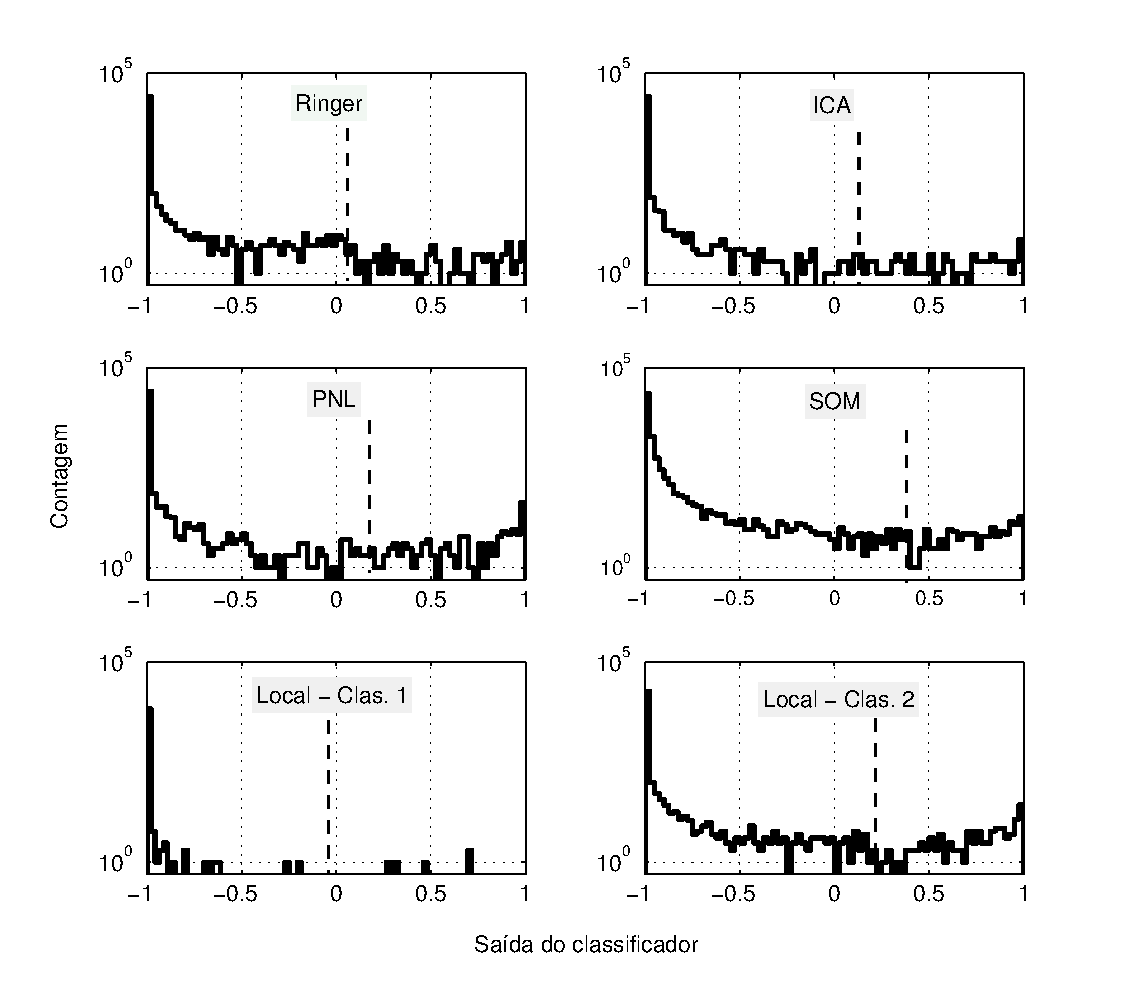
\epsfig{file=cosmics-net-out6,width=15cm}}
\end{minipage}
\caption{Saídas dos classificadores neurais para eventos de raios cósmicos.}\label{figcosmicNNo}
\end{figure}

Por fim, são apresentadas as eficiências na rejeição dos raios
cósmicos em função da energia, $\eta$ e $\phi$ para os diferentes
discriminadores. Considerando a energia, observa-se que o T2Calo
apresenta uma flutuação muito maior que os outros discriminadores.
Comparando os discriminadores neurais, observa-se que o pré-processamento
por ICA/NLICA produz uma eficiência aproximadamente constante, reduzindo a
flutuação em relação ao \emph{Neural Ringer}. Resultados semelhantes são
observados para as outras duas grandezas ($\eta$ e $\phi$).

\begin{figure}[h!]
\begin{minipage}[b]{0.98\linewidth}
  \centering
 \centerline{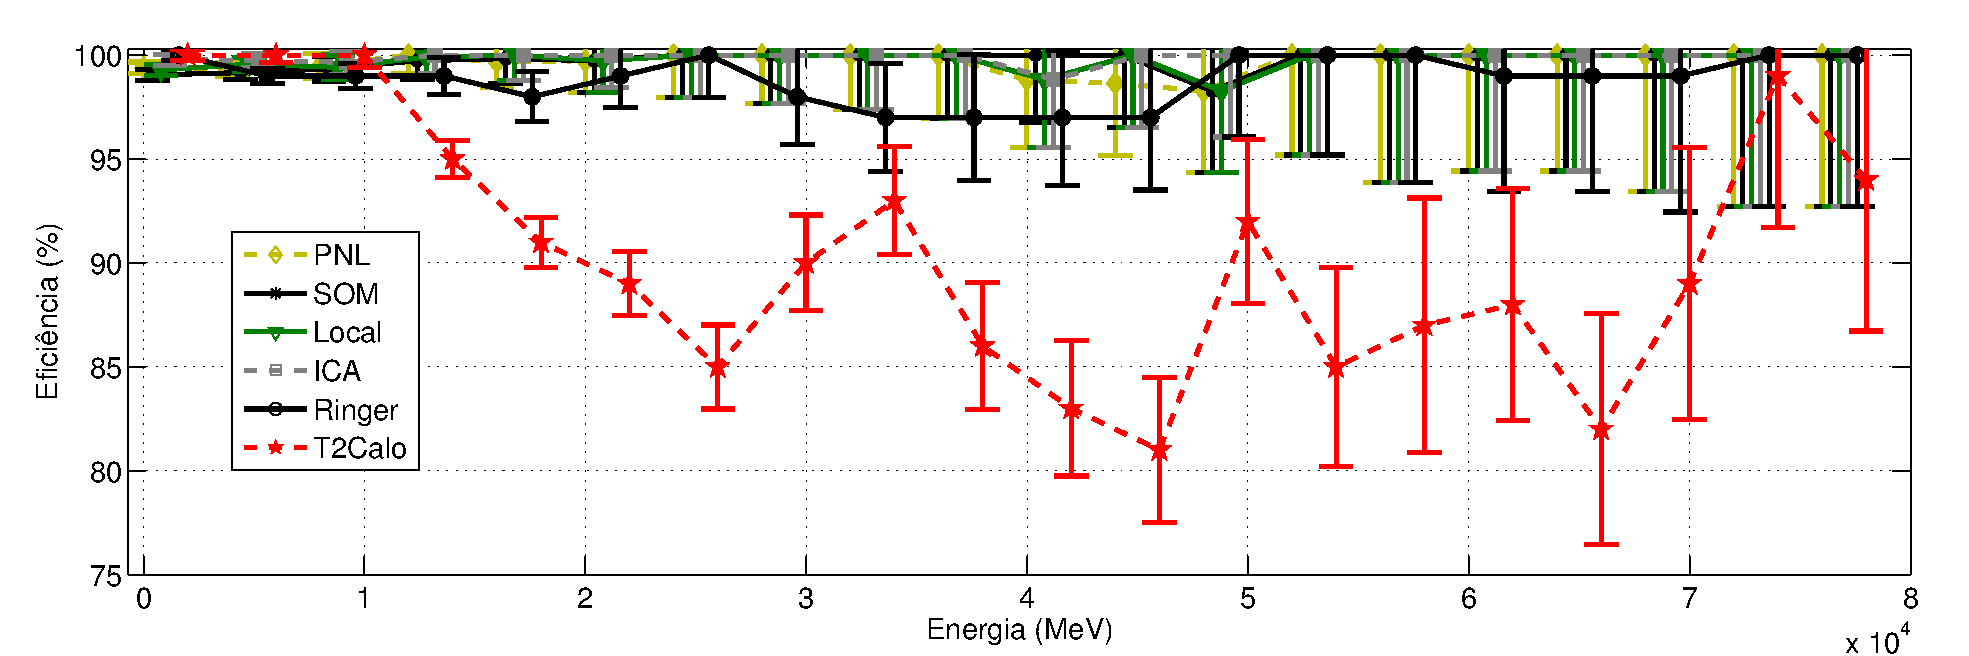
\epsfig{file=cosmic-comp-ef-et2,width=16cm}}
\end{minipage}
\hfill
\begin{minipage}[b]{0.98\linewidth}
  \centering
 \centerline{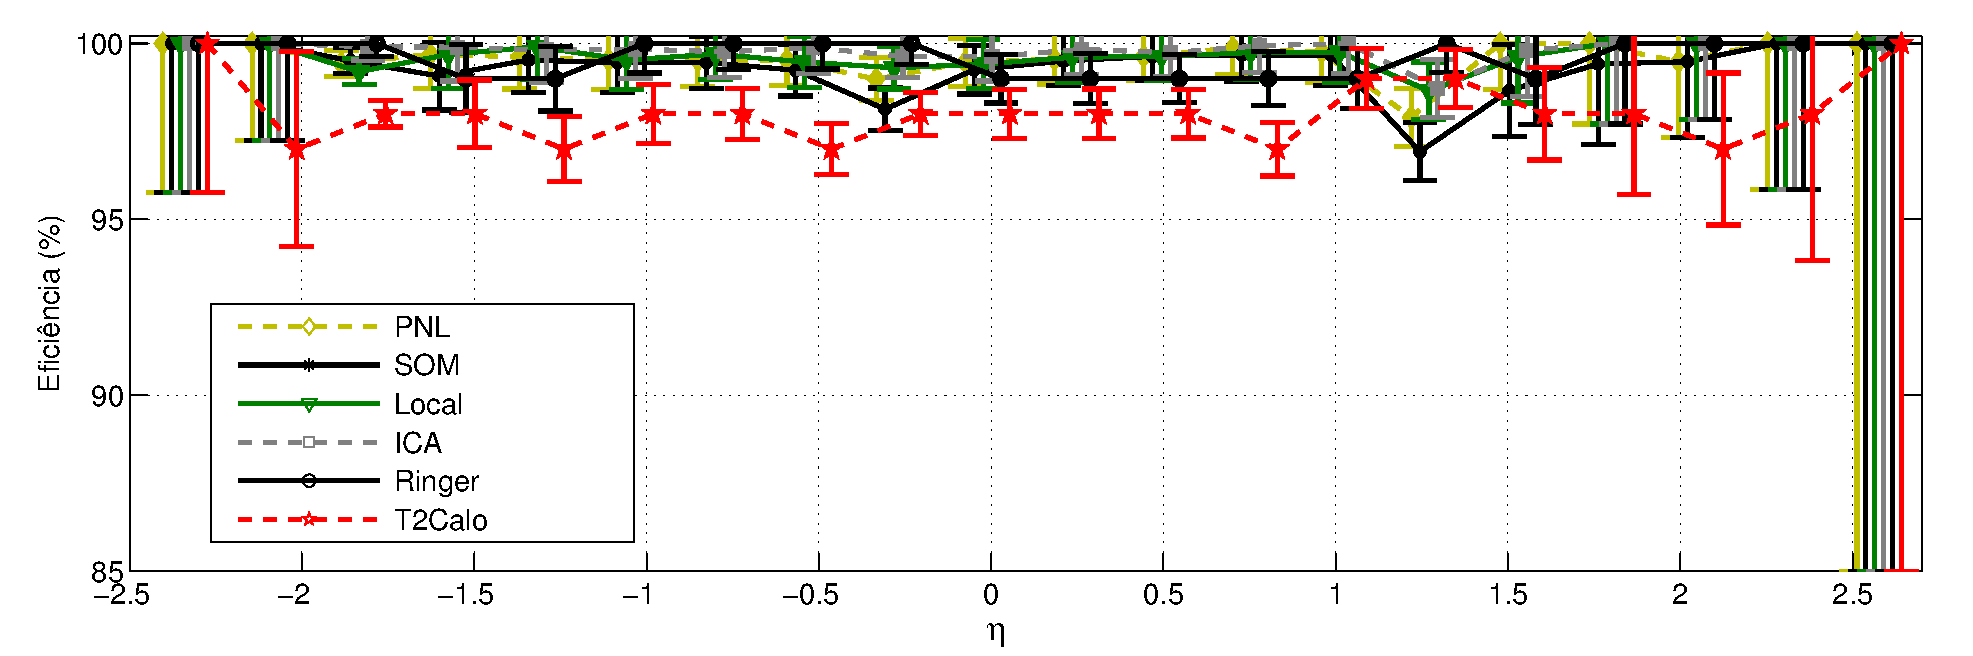
\epsfig{file=cosmic-comp-ef-eta2,width=16cm}}
\end{minipage}
\hfill \linebreak
\begin{minipage}[b]{0.98\linewidth}
  \centering
 \centerline{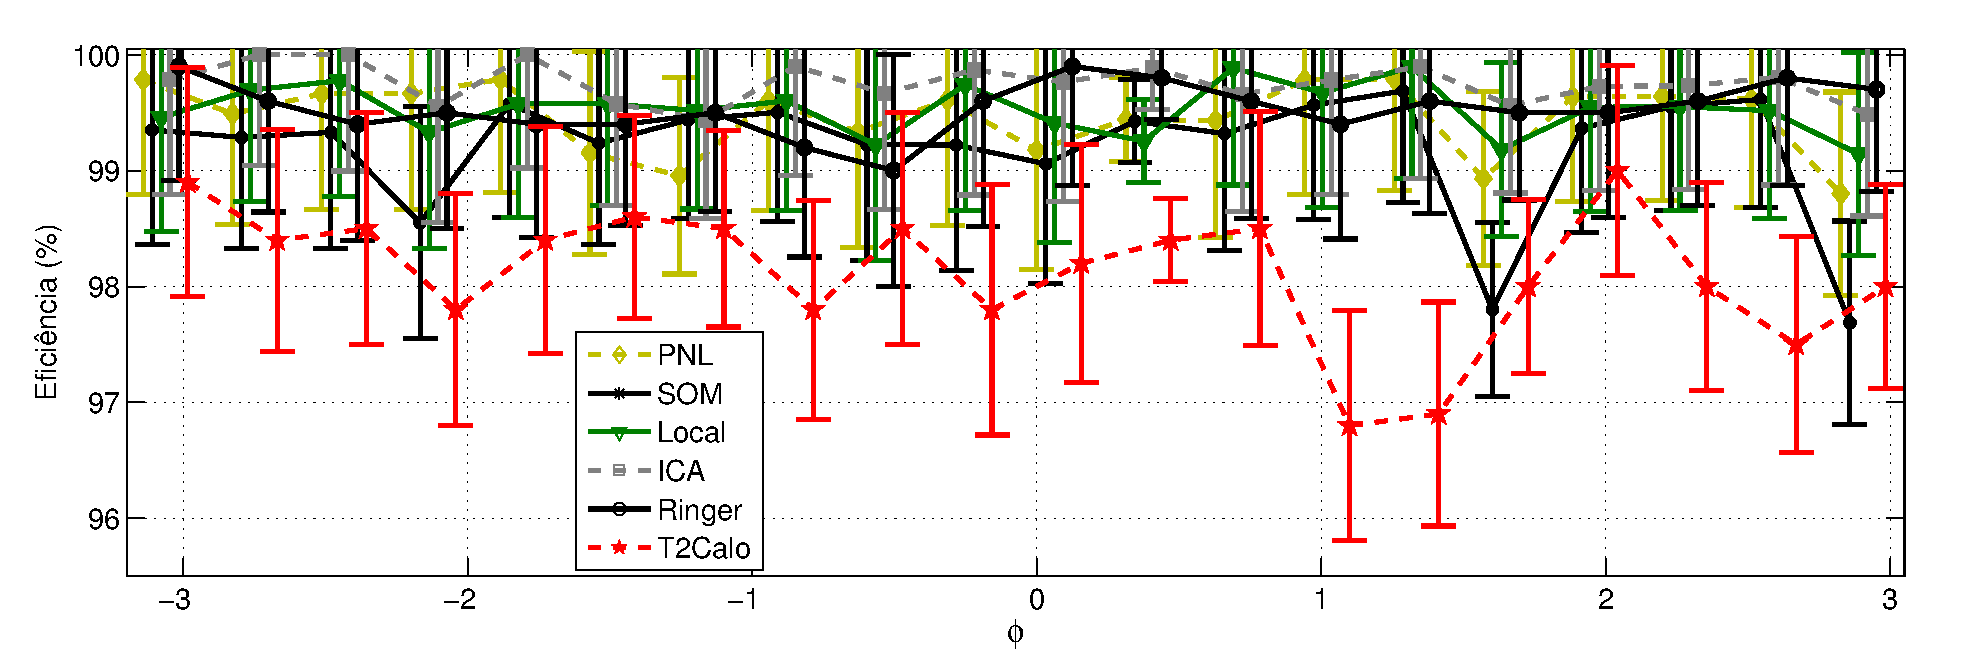
\epsfig{file=cosmic-comp-ef-phi2,width=16cm}}
\end{minipage}
\caption{Histogramas em energia $\eta$ e $\phi$ dos eventos de
raios cósmicos para diferentes discriminadores.}\label{figcosmicEF}
\end{figure}


\section{Sinais de Colisões do LHC}

Em sua fase inicial de operação (que deve durar até 2011), o LHC
irá operar com energias mais baixas do que a nominal (que é de
aproximadamente 14 TeV). Nos dados mais recentes, a energia máxima
das colisões está limitada em 7~TeV, 3,5~TeV por cada feixe (que,
embora represente apenas metade da energia de projeto do LHC, já é
um valor sete vezes maior que o antigo recorde mundial, que
pertencia ao acelerador Tevatron do Fermilab desde 2001).

Nos sinais experimentais não há a caracterização prévia do tipo de
partícula (como havia nos sinais simulados). Neste caso, foram
utilizadas informações obtidas da reconstrução \textit{offline},
que indicam a probabilidade de um certo evento ser ou não um
elétron. Neste estudo, foram considerados como elétrons os eventos
aprovados no critério \emph{electron medium} do \textit{offline}
(estes eventos tem alta probabilidade de serem realmente
elétrons). Para o conjunto dos jatos, foram utilizados os eventos
que não passaram no critério \emph{electron loose} do
\textit{offline} (são eventos com probabilidade muito baixa de
serem elétrons). Ao todo, os conjuntos de prováveis elétrons e
jatos são formados respectivamente por 74.549 e 2.322.048
assinaturas. Estes eventos foram filtrados pelo primeiro nível
através de um corte em energia na faixa de 3~GeV (não foram
aplicados cortes de isolamento).

Na Figura \ref{fig_carexp}, pode-se observar que os eventos (para
ambas as classes) estão concentrados entre 2,5 e 7~GeV, embora
alguns (poucos) eventos cheguem a 15~GeV ou mais. Analisando as
distribuições em $\eta$, percebe-se que, a concentração em torno
de $|\eta|\sim 1,5$ é bastante reduzida. Isso se deve,
provavelmente, pela seleção baseada nos critérios da reconstrução
\emph{offline}, pois, como os eventos na região do \emph{crack}
têm uma amostragem mais grosseira (devido ao menor número de
células sensoras), eles podem não ser aprovados em nenhum dos
critérios utilizados. As distribuições em $\phi$ tem um
comportamento mais uniforme.

\begin{figure}[bth]
\begin{minipage}[b]{0.48\linewidth}
  \centering
 \centerline{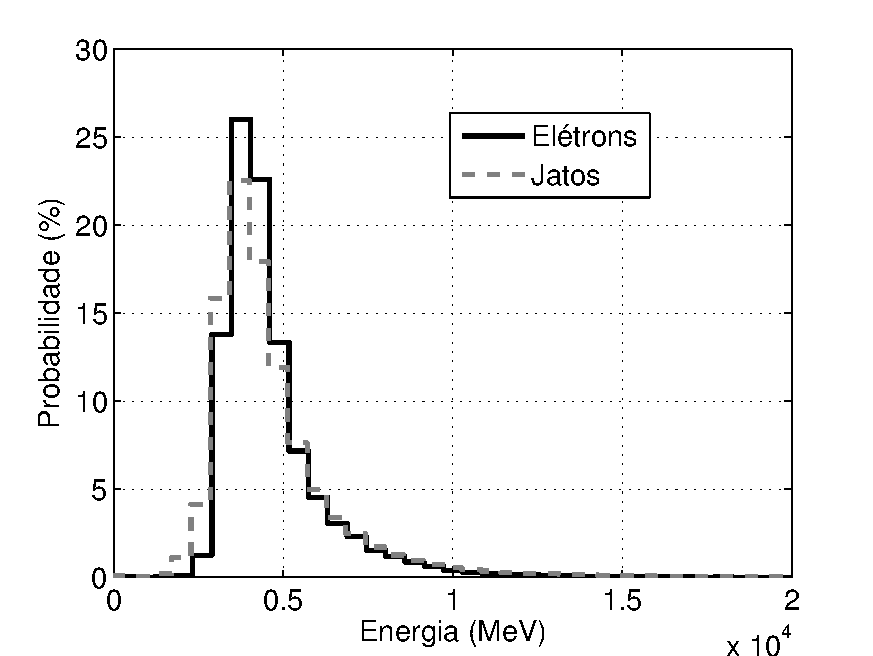
\epsfig{file=exp_et,width=8cm}}
\end{minipage}
\hfill
\begin{minipage}[b]{0.48\linewidth}
  \centering
 \centerline{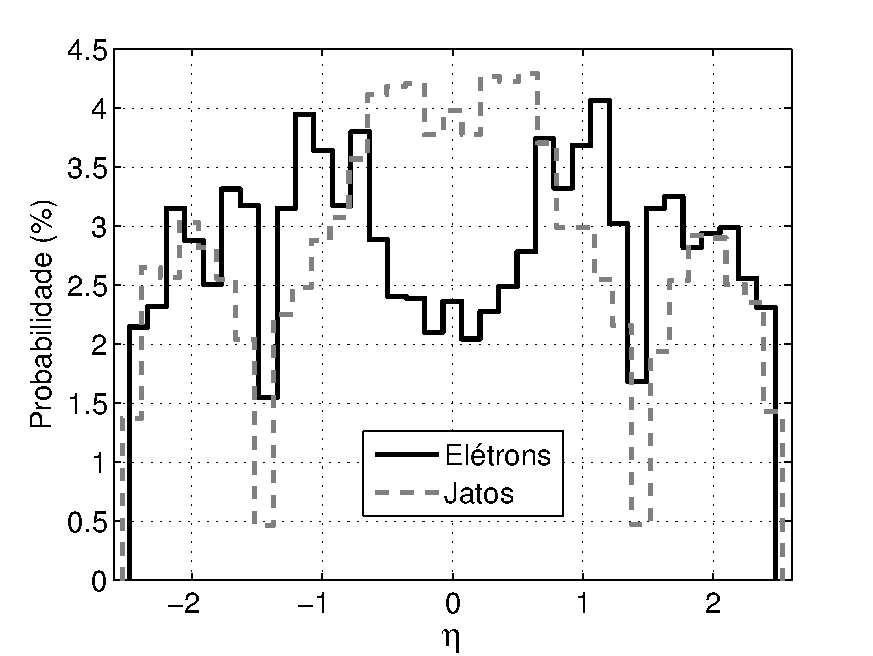
\epsfig{file=exp_eta,width=8cm}}
\end{minipage}
\hfill \linebreak
\begin{minipage}[b]{0.98\linewidth}
  \centering
 \centerline{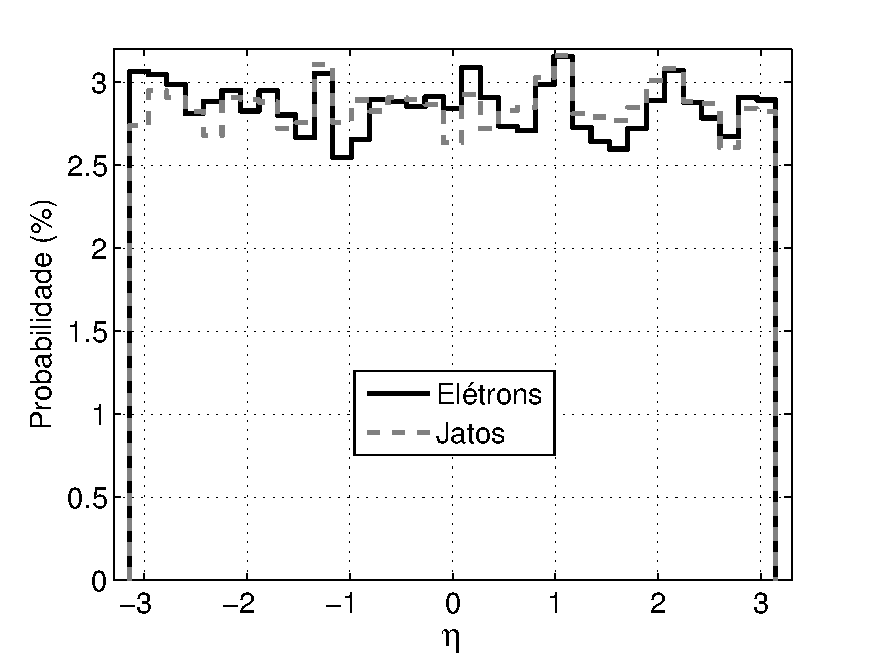
\epsfig{file=exp_phi,width=8cm}}
\end{minipage}
\caption{Histogramas em energia $\eta$ e $\phi$ dos eventos de
colisões do LHC.}\label{fig_carexp}
\end{figure}

As características dos perfis de deposição de energia medidos nos
calorímetros também dependem da energia dos eventos. Conforme
mostrado anteriormente no Capítulo~\ref{cap_atlasEtrig}, as razões
$\frac{E_{HAD}}{E_{EM}}$ e $\frac{E_{3 \times 7}}{E_{7 \times 7}}$
(importantes na separação elétron/jato) se modificam bastante em
baixa energia, tornando mais difícil a identificação das
partículas. Outro aspecto a ser considerado é a resolução relativa
dos calorímetros, que também é função da energia, conforme a
expressão~\cite{book:wigmans:2000}:
\begin{equation}\label{eq_erExp}
 \frac{\sigma_E}{E}=\frac{a}{\sqrt{E}}+b.
\end{equation}
A expressão da Equação~\ref{eq_erExp} não considera o ruído
eletrônico, que é proporcional a $1/\sqrt{E}$. Em testes
experimentais dos calorímetros do ATLAS (descritos detalhadamente
em~\cite{article:ATLAS:2008}) foram encontrados valores para os
parâmetros $a$ e $b$ da Equação~\ref{eq_erExp}. Para a seção
eletromagnética obteve-se $a=10,0\%.\sqrt{\text{GeV}}$ e
$b=0,17\%$ e para a hadrônica $a\sim 21,4 \%.\sqrt{\text{GeV}}$ e
$b\sim 0 \%$. Com estes valores, na Tabela~\ref{tab_res_exp},
foram estimadas as resoluções esperadas para as duas seções do
calorímetro com energia variando de 3 a 40 GeV, pode-se observar
que, na faixa de energia dos sinais experimentais ($\sim$3GeV) a
resolução é aproximadamente 2,5 vezes pior do que em 20~GeV.

\begin{table}[h!]
\centering \caption{Resolução relativa ($\frac{\sigma_E}{E}$ em \%) em função da energia.}\vspace{0.2cm} \footnotesize
\begin{tabular}{c|c|c|c}
    \hline
\textbf{Energia (GeV)} & \textbf{3} & \textbf{20} & \textbf{40} \\
\hline
\textbf{Cal. EM} & 12,4 & 4,8 & 3,4 \\
\textbf{Cal. HAD} & 5,9 & 2,4 & 1,8 \\
\hline
\end{tabular}
\label{tab_compTimeexpSeg}
\end{table}

Um comparativo entre os eventos médios do conjunto simulado (corte
E10) e dos sinais experimentais é apresentado na
Figura~\ref{fig_exp_compEvMed}. Como a implementação do
\emph{Ringer} na plataforma de software do ATLAS utilizava, no
momento da aquisição dos dados, a normalização sequencial, os
eventos são mostrados neste formato. Pode-se observar que, os
eventos experimentais de elétrons tem, em média, maior energia
hadrônica e menor concentração espacial se comparados aos
simulados. Considerando os jatos, as diferenças são um pouco
menores, porém, pode-se notar uma menor intensidade de energia
hadrônica nos sinais experimentais. Deste modo, os sinais
experimentais das duas classes apresentam maior semelhança, o que
torna mais difícil sua separação.

\begin{figure}[th]
\begin{minipage}[b]{0.48\linewidth}
  \centering
  \centerline{\footnotesize Elétrons/Simulados-E10}\medskip
 \centerline{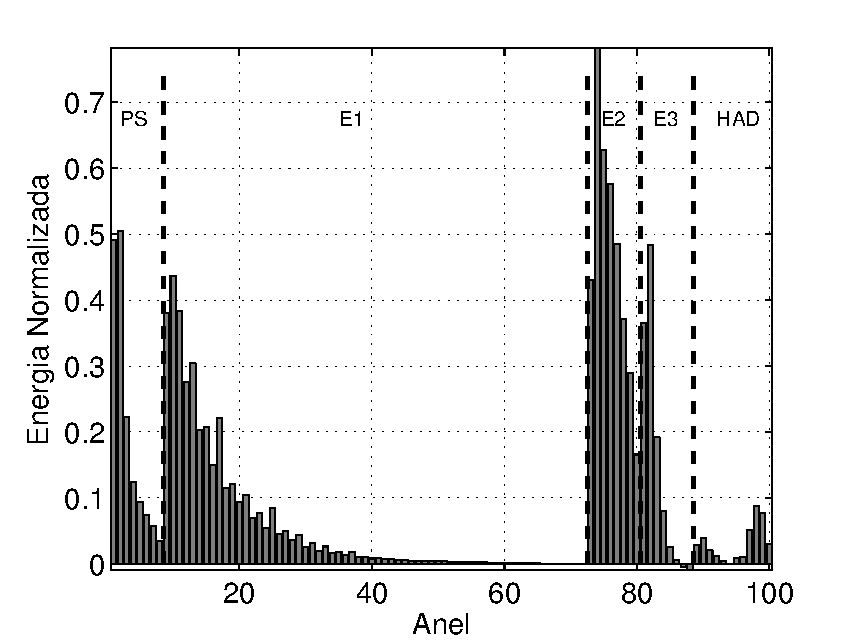
\epsfig{file=e10_evmedEseq,width=7cm}}
\end{minipage}
\hfill
\begin{minipage}[b]{0.48\linewidth}
  \centering
  \centerline{\footnotesize Jatos/Simulados-E10}\medskip
 \centerline{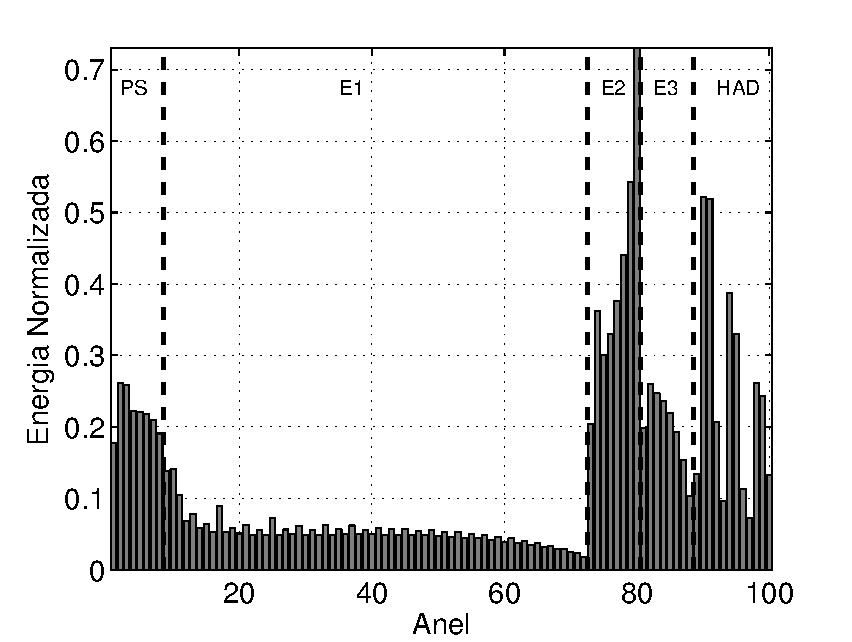
\epsfig{file=e10_evmedJseq,width=7cm}}
\end{minipage}
\hfill \linebreak
\begin{minipage}[b]{0.48\linewidth}
  \centering
  \vspace{.4cm}
  \centerline{\footnotesize Elétrons/Colisões}\medskip
 \centerline{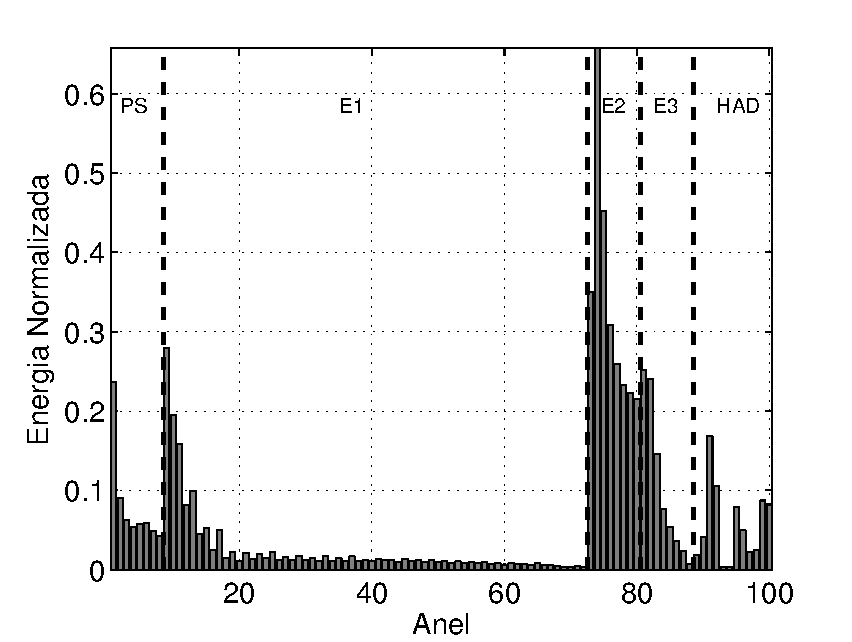
\epsfig{file=exp_evmedE,width=7cm}}
\end{minipage}
\hfill
\begin{minipage}[b]{0.48\linewidth}
  \centering
  \vspace{.4cm}
  \centerline{\footnotesize Jatos/Colisões}\medskip
 \centerline{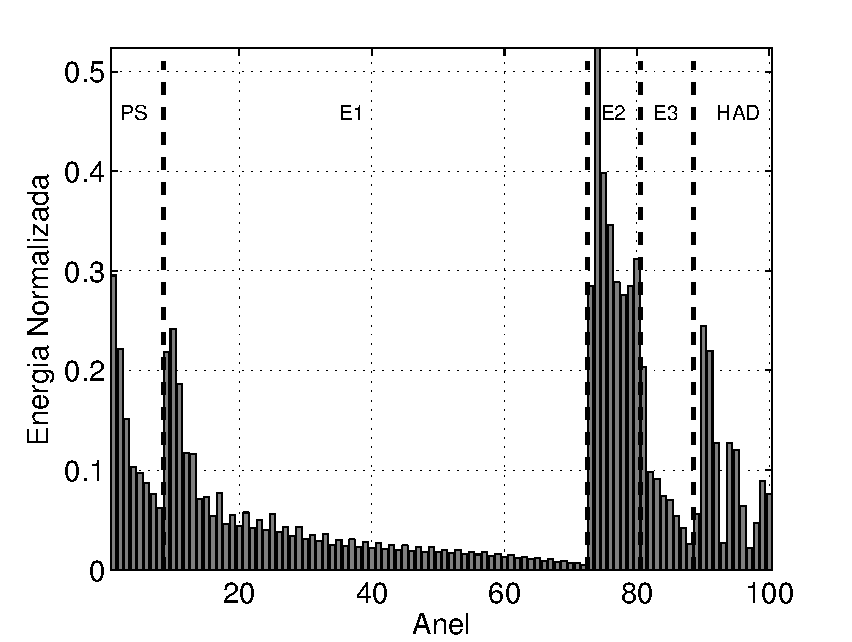
\epsfig{file=exp_evmedJ,width=7cm}}
\end{minipage}
\caption{Comparativo entre os eventos médios para o conjunto simulado-E10 (acima) e
os sinais experimentais (abaixo).}\label{fig_exp_compEvMed}
\end{figure}

Conforme mostrado, os sinais experimentais disponíveis até o
momento tem características físicas bem distintas dos sinais
simulados utilizados para desenvolvimento dos discriminadores.

Deste modo, aplicando-se diretamente aos sinais experimentais a
versão do \emph{Neural Ringer} treinada para o conjunto simulado
E10 é obtida uma eficiência de apenas 21,73~\%, para um falso
alarme igual a 19,50~\%. A Figura~\ref{fig_exp_RoutE10} mostra as
saídas do classificador neural. Pode-se observar que, as
distribuições dos eventos de elétrons e jatos é bem semelhante,
com uma maior concentração perto de -1.

\begin{figure}[htb]
\centering
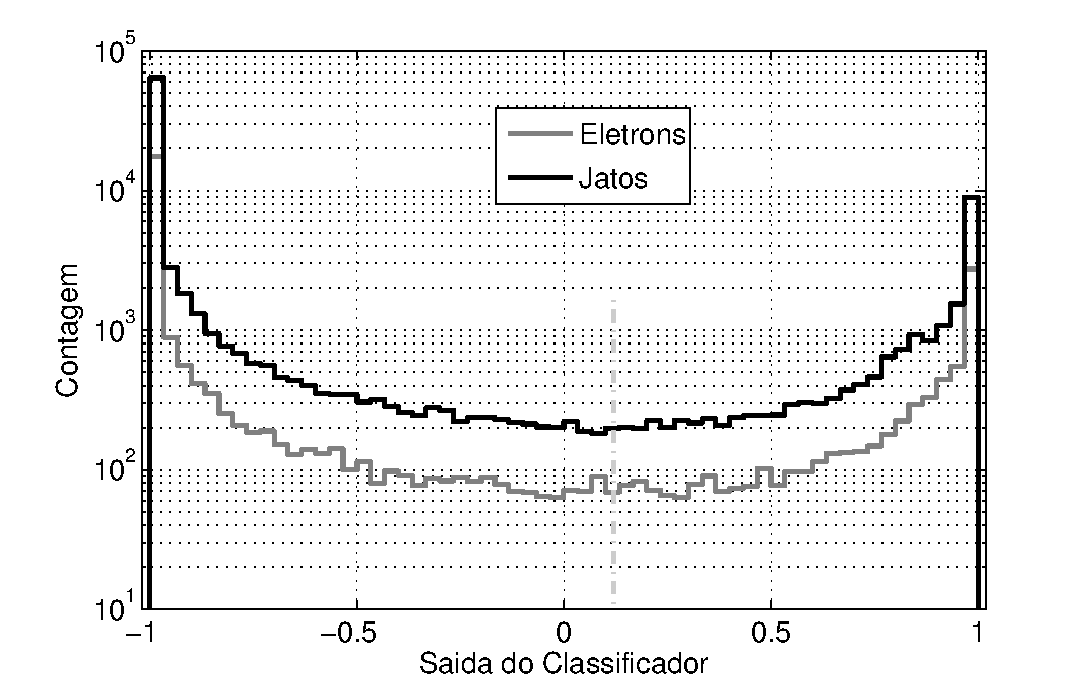
\includegraphics[width=10cm]{exp_out_ringerE10}
\caption{Saídas do \emph{Neural Ringer} (treinado para os sinais
simulados E10) para os sinais experimentais.}
\label{fig_exp_RoutE10}
\end{figure}

 Neste contexto, para melhor avaliar o desempenho das
técnicas de pré-processamento propostas neste trabalho, o processo
de treinamento será repetido, utilizando agora os sinais
experimentais. A informação da reconstrução \emph{offline} será
utilizada como ``verdade" para o treinamento. Para treinamento dos
classificadores foi utilizado um procedimento semelhante ao
descrito no Capítulo~\ref{cap_metod}.

\subsection{Resultados - Anéis}

Inicialmente, foi realizado um estudo para determinar se, no
contexto dos sinais experimentais, o número de neurônios ocultos
utilizado como padrão para os sinais simulados (10 neurônios)
também se mantém como uma boa opção para o caso experimental.
Foram treinadas várias redes, variando-se o número de neurônios
ocultos de 6 a 30. Para cada nova configuração foram realizadas 10
inicializações distintas, selecionado-se aleatoriamente a
composição dos conjuntos de treino, teste e validação. A
Figura~\ref{fig_exp_nh} mostra que o melhor SP foi obtido para uma
rede de 12 neurônios ocultos. Este número será usado como
referência para os discriminadores treinados com os sinais
experimentais.

\begin{figure}[htb]
\centering
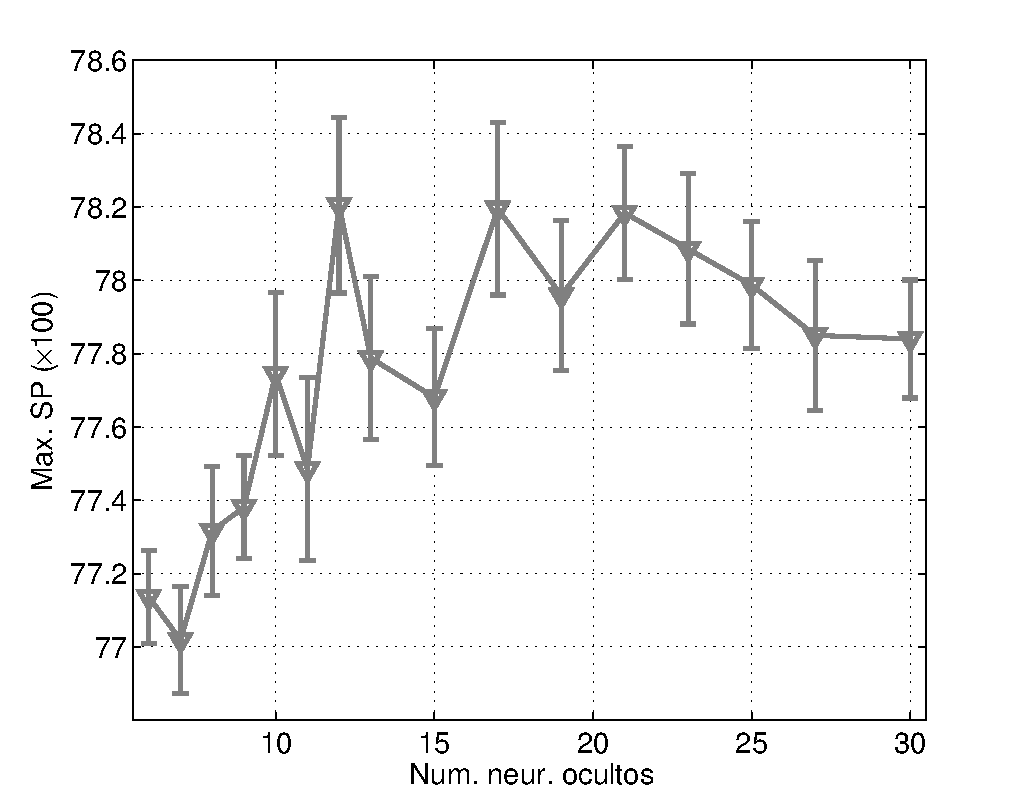
\includegraphics[width=10cm]{exp_estudo_sp_nh}
\caption{Máximo SP (média e desvio padrão) obtidos variando-se o número de neurônios ocultos.}
\label{fig_exp_nh}
\end{figure}

\subsection{Resultados - ICA}

\subsection{Resultados - NLICA}

\section{Estimativa do custo computacional dos algoritmos
propostos}

Conforme detalhado na seção \ref{sec_tempoR}, o \textit{Neural
Ringer} está implementado na plataforma de \textit{software} do
ATLAS como uma sub-rotina do T2Calo e seu fluxo de processamento
envolve as etapas a seguir:
\begin{enumerate}
    \item \textbf{Seleção de região} (T2Calo) - são selecionados os
    dados utilizados pelo T2Calo (0,4927$\pm$0,0787)~ms;
    \item \textbf{Pré-processamento} (T2Calo) - as variáveis de decisão do
    T2Calo são calculadas (0,1408$\pm$0,0148)~ms;
    \item \textbf{Seleção de região} (\emph{Ringer})  - são selecionados os
    dados utilizados pelo \textit{Neural Ringer} (0,4375$\pm$0,0996)~ms;
    \item \textbf{Anelamento} - construção dos anéis (0,0986$\pm$0,0165)~ms;
    \item \textbf{Normalização} - o vetor com os anéis é normalizado (0.0026$\pm$0,0015)~ms;
    \item \textbf{Classificação Neural} - a rede neural produz a decisão
    de aceitação/rejeição do evento (0,0387$\pm$0,0018)~ms.
\end{enumerate}
Em conjunto, as seis etapas totalizam (1,2109$\pm$0,1288)~ms.

Com o uso de uma etapa de pré-processamento para a classificação
neural (através da NLICA), é necessário verificar o efeito desta
modificação no tempo total para tomada de decisão.

As rotinas para operação da ICA Local e do modelo PNL foram
implementadas no sistema de filtragem do ATLAS e seu custo
computacional avaliado a partir da propagação de um conjunto de
eventos através das duas cadeias de processamento. Nesta
avaliação, as etapas de 1 a 5 do fluxo do \textit{Neural Ringer}
não são modificadas. Apenas na etapa 6, é adicionado o
pré-processamento para a rede neural.

No caso da ICA Local, a etapa 6 é constituída de 3 procedimentos:
\begin{enumerate}
    \item \textbf{Seleção do cluster} - as assinaturas que chegam
    são divididas nos dois clusters a partir do cálculo da
    distância (euclidiana) para o centro de cada cluster;
    \item \textbf{ICA$+$Rede Neural} - dentro de cada cluster, as
    assinaturas são projetadas nos componentes independentes e
    propagadas através da rede classificadora;
    \item \textbf{Comparação com o patamar} - as saídas das redes são
    comparadas com os patamares de decisão, produzindo a
    classificação propriamente dita.
\end{enumerate}
O tempo médio gasto em cada uma das etapas foi respectivamente
(0,0183$\pm$0,0037)~ms, (0,0474$\pm$0,0059)~ms e
(0,0081$\pm$0,0045)~ms, totalizando (0,0738$\pm$0,0083).

Para o modelo PNL, dois procedimentos substituem a etapa 6:
\begin{enumerate}
    \item \textbf{PNL-ICA$+$Rede Neural} - os sinais são mapeados
    nos componentes independentes e propagados pela rede
    classificadora;
    \item \textbf{Comparação com o patamar} - a saída da rede é
    comparada com o patamar de decisão.
\end{enumerate}
As etapas acima foram completadas respectivamente em
(0,0747$\pm$0,0074)~ms e (0,0067$\pm$0,0043)~ms, totalizando
(0,0814$\pm$0,0085)~ms.

A Tabela~\ref{tabExpTempo} resume os resultados mostrados acima,
incorporando também o tempo total dos discriminadores e uma
comparação (percentual) com o tempo gasto pelo \textit{Neural
Ringer}. Observa-se que, o uso do pré-processamento por NLICA
contribui pouco para o aumento do custo computacional, implicando
em apenas 2,90\% e 3,53\% de aumento em relação ao \textit{Neural
Ringer}, respectivamente para a ICA Local e a PNL-ICA.

\begin{table}[h!]
\centering \caption{Comparação dos tempos de processamento para
diferentes discriminadores.}\vspace{0.2cm} \footnotesize
\begin{tabular}{c|c|c|c}
    \hline
\textbf{Discriminador} & \textbf{Prep.+Classif. Neural} (ms)&
\textbf{Total} (ms) & \% do \textit{Ringer} \\
\hline
T2Calo & - & 0,6469$\pm$0,0802 & 53.42\\
\textit{Neural Ringer} & 0,0387$\pm$0,0018 & 1,2109$\pm$0,1288 & 100,00\\
Local ICA$+$MLP & 0,0738$\pm$0,0083 & 1,2460$\pm$0,1520 & 102,90\\
PNL $+$ MLP & 0,0814$\pm$0,0085 & 1,2536$\pm$0,1526 & 103,53\\
\hline
\end{tabular}
\label{tabExpTempo}
\end{table}


\subsection{Abordagens segmentadas}

\begin{table}[h!]
\centering \caption{Comparação de desempenho para diferentes
discriminadores, corte E10.}\vspace{0.2cm} \footnotesize
\begin{tabular}{c|c|c|c | c}
    \hline
\textbf{Camada} & \textbf{Seleção da RoI} & \textbf{Anelamento} &
\textbf{Total} & \%\textbf{do total} \\ \hline
PS & 0,0071$\pm$0,0018 & 0,0091$\pm$0,0044 & 0,0162$\pm$0,0047 & 2,2\\
E1 & 0,1264$\pm$0,0309 & 0,0311$\pm$0,0077 & 0,1575$\pm$0,0318 & 21,8\\
E2 & 0,0794$\pm$0,0091 & 0,0203$\pm$0,0021 & 0,0997$\pm$0,0093 & 13,8\\
E3 & 0,0425$\pm$0,0056 & 0,0111$\pm$0,0018 & 0,0536$\pm$0,0059 & 7,4\\
H0 & 0,1230$\pm$0,0775 & 0,0080$\pm$0,0029 & 0,1309$\pm$0,0776 & 18,1\\
H1 & 0,1214$\pm$0,0775 & 0,0071$\pm$0,0027 & 0,1285$\pm$0,0776 & 17,8\\
H2 & 0,1292$\pm$0,0778 & 0,0071$\pm$0,0018 & 0,1364$\pm$0,0778 & 18,9\\
\hline
\end{tabular}
\label{tab_compTimeexpSeg}
\end{table}
